\subsection{Autoethnographic Research-Creation with Collaborative Validation}

This study employs an autoethnographic angle to its research-creation design, along with small-cohort collaborative validation. The primary unit of investigation is my own practice, as a Black scholar-practitioner, modifying both tools and modes of the practice through three iterative solo works that function as the "research instruments." These will serve as active sites where cultural knowledge and technical constraint friction into new procedural knowledge. The autoethnographic approach is essential because embodied, culturally specific tacit knowledge cannot be adequately accessed through observation alone; it requires first-person engagement with the full affective, sensorial, and decision-making dimensions of tool modification. This positions the research within what Loveless describes as a "driven, erotic, uncanny orientation" where inquiry follows "the desires articulating the eruptions of the drive(s)" that emerge through making \parencites[105]{Loveless_2019}. The researcher's body, listening practices, and technical decision-making become both the site and the apparatus of knowledge production.

However, autoethnography alone risks running rampant of solipsism or egotism. Sengers et al. identify this as the danger of designers remaining trapped in their own "blind spots" without mechanisms for critical reflection \parencites[49]{Sengers_2005}. Because of this potential danger, the design incorporates small-cohort workshops as structured sites for the Transmitting and Intimate Witnessing phases of ST, where modifications are tested for cultural resonance, technical documentation is refined, and collective reflection generates insights that exceed individual practice. 

One important distinction here is these are not meant to serve, specifically, as sites of collaborative art-making; I retain sole authorship of the three works and sole responsibility for their technical modifications and implementations. Rather, cohort members function primarily as "cultural validators," positioned to evaluate whether modifications successfully encode intended cultural logics and to surface assumptions I cannot see from within my own practice. This may take the form of embodied engagement with works or extracted modifications and processes of the research instruments. However, they will not directly build or modify the final works.

\subsection{Methodological Integration: Conventional Methods within ST}

The organizing structures of ST does not attempt to replace conventional research methods. Rather, what it does is engage in polydisciplinamory and provides an organizing framework for those other methods and procedures to be culturally accountable with integration. Table \ref{tab:methods-st} maps conventional methods to ST processes, showing how established approaches from HCI, design research, and arts-based inquiry are actualized within each cycle phase. Autoethnography provides first-person documentation during Embodying; critical technical practice surfaces embedded assumptions during Unsettling; reflective and speculative design guide prototype directions from Unsettling through Remixing; participatory approaches inform Transmitting and validation; research-through-design animates the entire Remixing and Embodying arc; and embodied inquiry evaluates experiential adequacy. Rather than describing each method in isolation, the following subsections detail how these approaches function within the study's primary and secondary components, emphasizing their roles in generating and validating culturally grounded modifications.

\begin{figure}[H]
	\centering
	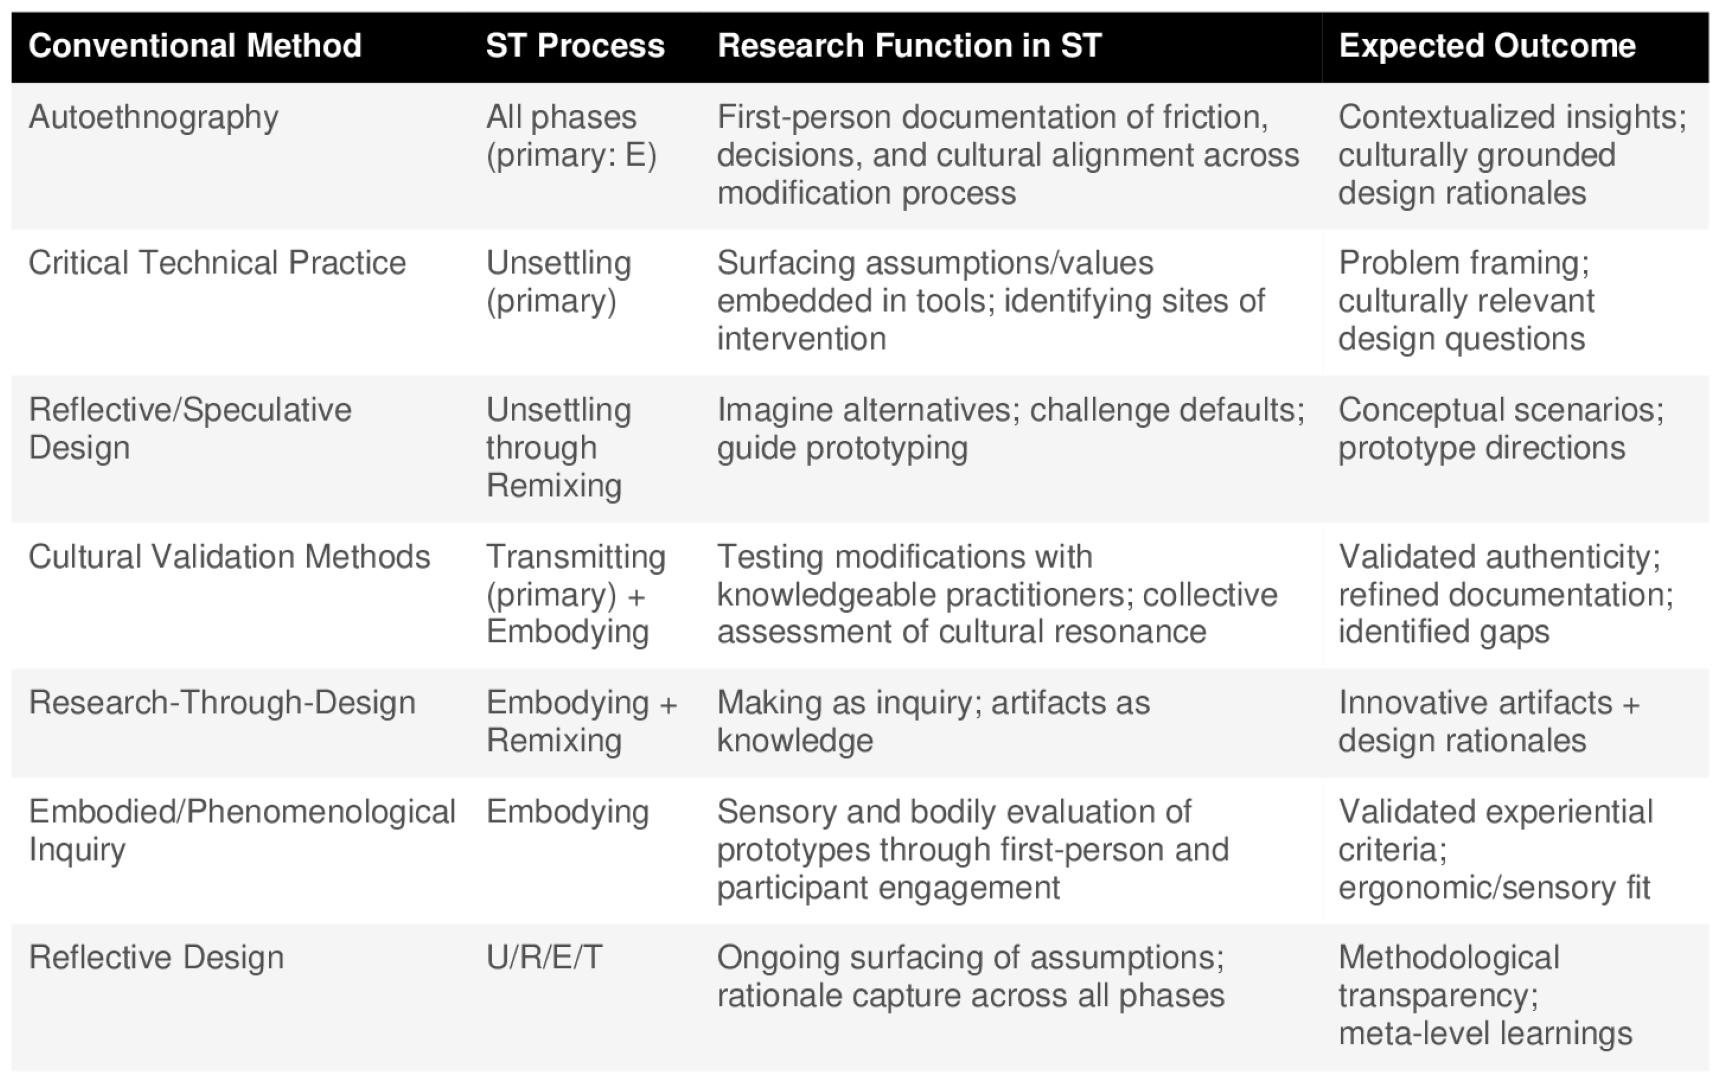
\includegraphics[width=1.0\textwidth]{assets/tables/table_3_1_STMethods.png}
	\captionof{table}{Conventional methods mapped to ST processes and research functions}
	\label{tab:methods-st}
\end{figure}

\subsection{Primary Component: Solo Practice-Based Works as Research Instruments}

The study centers on three solo works—\emph{Buffalo Soldier}, \emph{Did Sun Ra Fear Cryosleep?}, and \emph{Don't Play with My Hair}—developed iteratively over 8-10 months. Each work enacts a complete ST cycle while engaging different material substrates and sonic interaction modalities as sites for tool modification.
 
\textit{Buffalo Soldier} investigates tactility and material substrate through modified spatialization techniques that encode historical memory and speculative narrative. 
\textit{Did Sun Ra Fear Cryosleep?} explores fluid dynamics and sedimentation through hydrophone-based interfaces that challenge conventional audio processing paradigms. 
\textit{Don't Play with My Hair} examines gestural and structural properties through a custom synthesizer architecture grounded in embodied habits.

ST's four domains operate as concurrent analytical filters applied throughout each work's complete cycle.  Each phase of each work is interrogated through all four domains simultaneously: What does this modification refute? OR how does it function "unintentionally?" (Fugitive Speculation)? How does it encode embodied and/or cultural memory (Material Memory)? Does it enable specific sensory interaction based on shared or lived experiences (Sensory Worlding)? How can it be transmitted with its cultural reasoning intact (Intimate Witnessing)?

These works are emergent research instruments the arise from the modification process itself. They are the aim, the "goal" of the research. They are not an existing artistic endeavor with the guise of research and of scholarly inquiry shoehorned onto them. As Loveless argues, research-creation refuses "monodisciplinary logics" and instead follows "driven curiosity as its lure and guide," allowing "practices to be responsive to the polymorphous nature of desire" while maintaining "rigorous accountability to the specific cultural epistemologies and material conditions that animate the work" \parencites[62, 105]{Loveless_2019}. The relationship between the works are intended to be cumulative and reflexive. Technical insights from one informs the processing approaches in another. Each works documentation challenges shape the transmission strategies developed for each other, iteratively. This recursive structure enacts what Manning and Massumi describe as "spiraling eternal return: always more than one" iteration, where later works inherit and transform earlier learnings while earlier works may be revisited with new technical understanding \parencites[131]{Manning_Massumi_2014}.

Each work generates both aesthetic artifacts (performances, sound installations, recordings) and methodological artifacts (modified code, documentation schemas, decision rationales) that together constitute the study's outputs. Detailed descriptions of each work's cultural grounding, sonic materials, and artistic trajectory are provided in Chapter \ref{ch:practice}.

\subsection{Secondary Component: Small-Cohort Sessions as Transmission Sites}

Approximately 3-5 planned small-cohort sessions aim to provide structured sites for Transmitting modifications and practicing Intimate Witnessing. Each session involves 1-5 participants recruited from Drexel's Westphal College of Media Arts \& Design, or from associated creative practitioners or research collective members in the greater Philadelphia, PA region who can evaluate modifications for cultural authenticity and experiential resonance. Potential collaborators include advanced graduate students, artists, designers, technologists, and faculty affiliates with both minimal technical fluency and deep engagement with/understanding of cultural aesthetics (not limited to only Black/Afro-diasporic aesthetics). This ensures participants can assess modifications at the intersection of cultural logic and technical implementation. Sessions are planned to be scheduled at key transition points within the ST cycle. (See the following suggested points of reflection):

\begin{enumerate}[nosep]
	\item Following Work 1's initial Embodying phase to validate early modifications before finalizing documentation;
	\item Between Works 1 and 2 to collectively reflect on transmission materials and refine modification procedures;
	\item Following Work 3 to assess the transmissibility of accumulated procedural knowledge.
\end{enumerate}

\textit{Additional sessions may be scheduled as needed based on emergent research demands.}

Again, these sessions are explicitly \textit{not} meant to be sites of collaborative art-making in the conventional sense. We aim to have collaborating scholar-practitioners engage modifications through hands-on testing, provide culturally grounded feedback on whether tools "feel right" in practice, and collectively reflect on the adequacy of documentation for cultural transmission. Session activities include:

\begin{enumerate}[nosep]
	\item \textbf{Structured hands-on engagement:} Participants use modified tools to create short improvisational sketches, generating experiential knowledge of how modifications constrain and enable practice;
	\item \textbf{Collective listening/movement exercises:} Assessment of whether spatial configurations support culturally specific embodied interactions (e.g., call-and-response structures, polyrhythmic layering);
	\item \textbf{Documentation review:} Participants attempt to implement modifications using only provided materials, revealing gaps in transmissibility;
	\item \textbf{Reflective dialogue:} Participants articulate what modifications accomplish culturally and what remains inadequately addressed.
\end{enumerate}

The small scale is intentional: larger groups would dilute the intimacy required for vulnerable knowledge sharing. This scale aligns with Manning and Massumi's "molecular" organizing, or networked pods of practitioners engaged in "emergent attunement" rather than mass participation \parencites[106-110]{Manning_Massumi_2014}.

\subsection{Data Collection and Documentation Practices}

Data collection occurs throughout all ST phases, with different artifact types foregrounded at each stage (see Table \ref{tab:data-by-stage}). 
\begin{itemize}[noitemsep]
	\item \textbf{Unsettling} comprises audit notes documenting embedded assumptions, screenshots of tool interfaces, friction logs recording moments of cultural misalignment, and annotated literature excerpts that frame cultural logics guiding modification decisions.
	\item \textbf{Remixing} generates versioned code repositories (with commit messages explaining rationale), design sketches exploring alternative parameter mappings, modified patches and plugins, and decision memos that document why specific technical choices encode specific cultural relations.
	\item  \textbf{Embodying} produces autoethnographic field notes capturing affective responses and experiential qualities of working with modifications, video/audio recordings of practice sessions showing embodied interaction patterns, screen recordings documenting workflow changes, and photographic documentation of physical setups and gestural techniques.
	\item \textbf{Transmitting} yields multiple documentation formats including annotated code with inline cultural explanations, tutorial videos demonstrating modification procedures, written technical guides with cultural rationales, and refined naming conventions/metadata schemas that make cultural reasoning legible to future practitioners.
\end{itemize}
  Across all phases, reflective notes will help to synthesize emergent insights, theoretical connections, and methodological adjustments, creating a meta-level documentation trail that tracks the evolution of ST as methodology alongside the development of each specific modification.

During the secondary collaborative component sessions, multiple forms of data parallel and extend primary component collection. Video documentation captures participants' embodied interactions with tools, revealing gestural and postural patterns that indicate whether spatial mappings align with cultural practices. Screen recordings document how participants navigate modified interfaces, showing whether naming conventions and parameter organizations prove intuitive or confusing. Collective note-taking during reflective dialogue produces collaborative interpretations that surface assumptions I cannot perceive from within my own practice. Audio recordings preserve verbal feedback and group discussions, while participants' improvisational sketches generated during hands-on engagement become artifacts demonstrating what modifications enable or foreclose in practice. These session data serve primarily as validation mechanisms: testing whether modifications achieve intended cultural effects and whether documentation successfully transmits modification procedures and their underlying reasoning.

\begin{figure}[H]
	\centering
	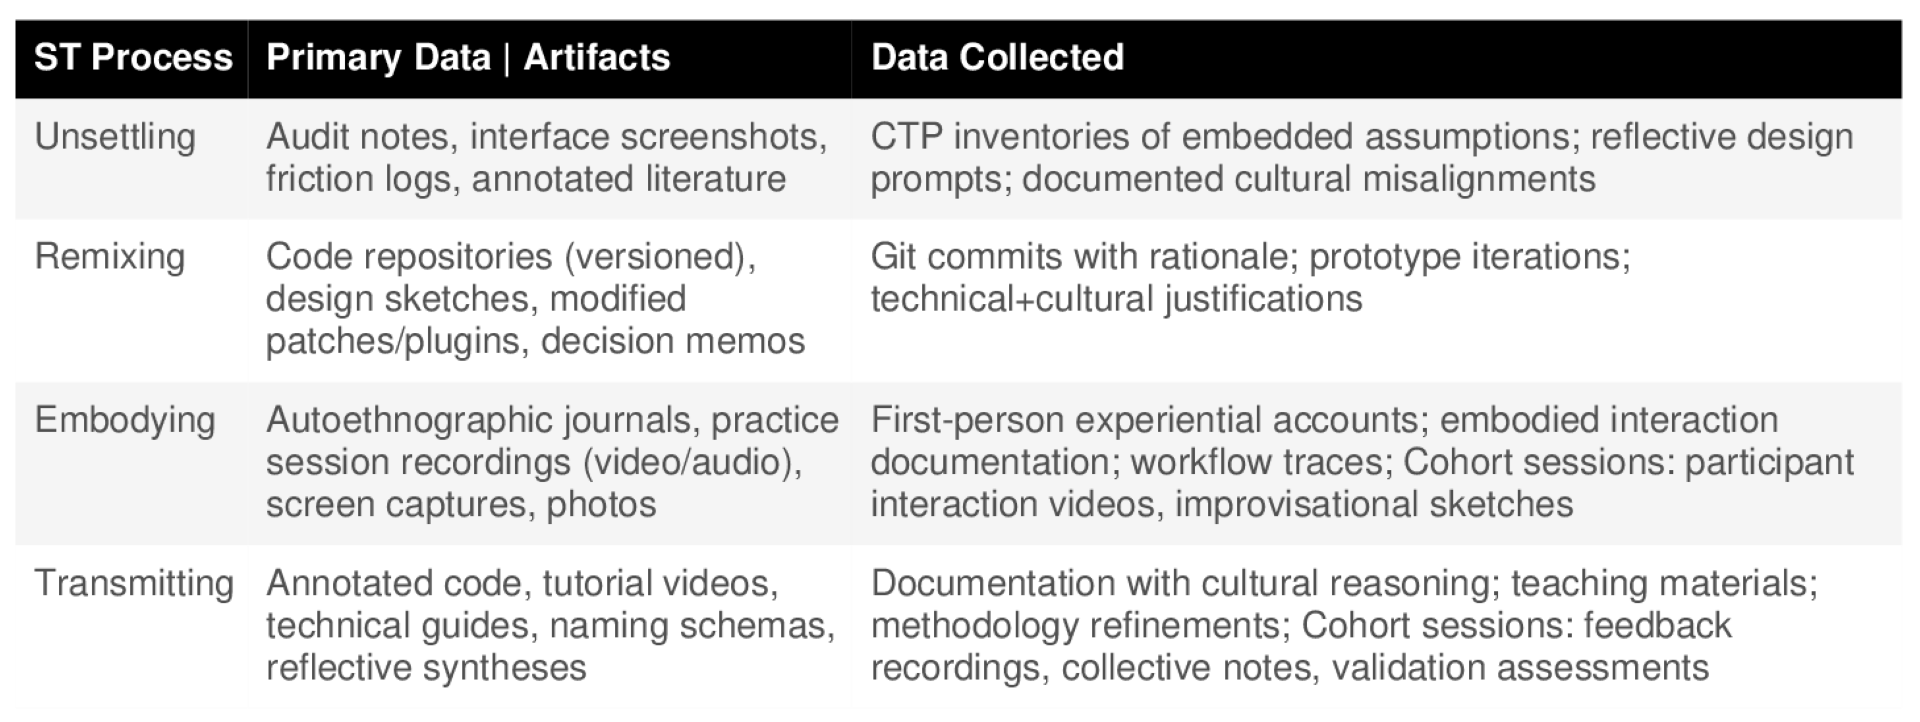
\includegraphics[width=1.0\textwidth]{assets/tables/table_3_2_Data.png}
	\captionof{table}{Data sources and artifacts by ST process}
	\label{tab:data-by-stage}
\end{figure}


\subsection{Units of Analysis and Evaluation Criteria}
Analysis focuses on four interconnected units that together demonstrate how ST generates transmissible procedural knowledge: (1) technical artifacts including modified code, custom parameter mappings, audio patches, and interface prototypes; (2) decision documentation comprising reflective memos, version-control commit messages, and annotated sketches that explain why specific modifications may encode specific cultural relations; (3) experiential accounts including autoethnographic field notes, video documentation of practice sessions, and cohort feedback that capture what modifications enable and foreclose in practice; and (4) transmission materials encompassing code documentation, tutorial demonstrations, naming conventions, and teaching protocols developed to make modifications implementable by others. Each unit is analyzed through ST's four domains (Fugitive Speculation, Material Memory, Sensory Worlding, Intimate Witnessing) to assess how successfully modifications resist dominant paradigms, encode cultural memory, enable culturally specific sensory interaction, and support accountable knowledge transmission.

The evaluation criteria described is intended to be qualitative, phenomenological, and culturally grounded as a reflection of the methodological underpinnings at at large.

\begin{figure}[H]
	\centering
	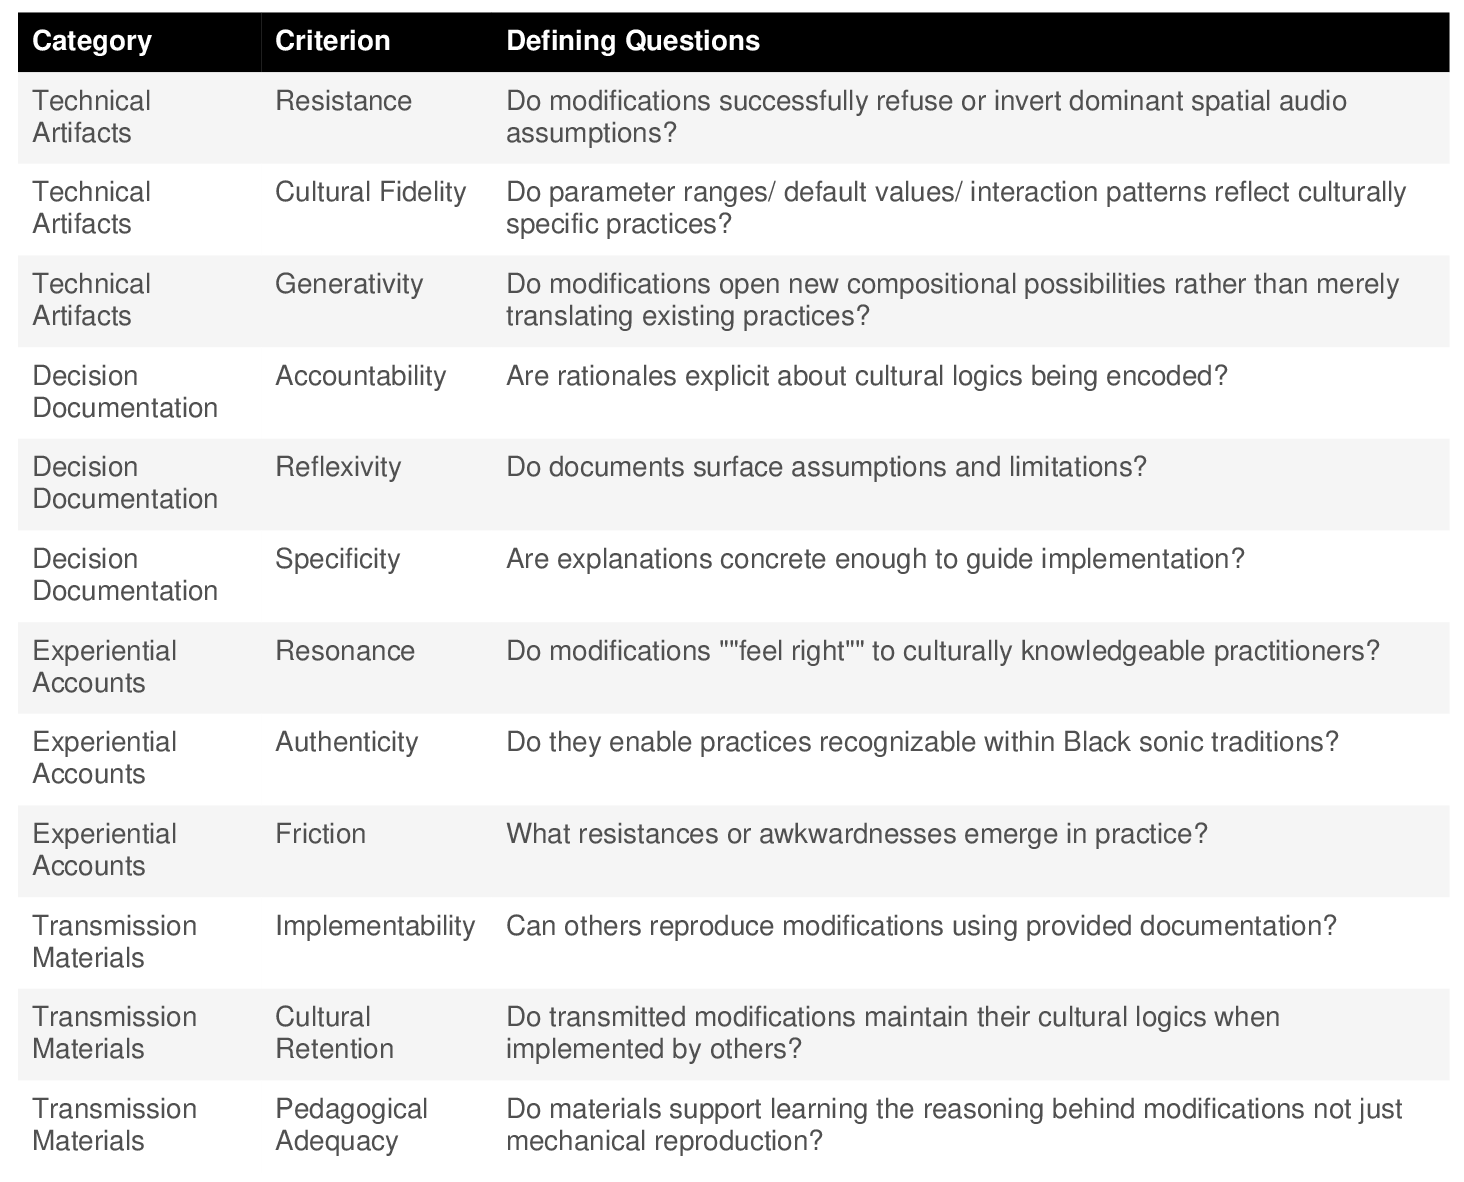
\includegraphics[width=1.0\textwidth]{assets/tables/table_3_3_evalCriteria.png}
	\captionof{table}{Evaluation criteria for data sources and types}
	\label{tab:eval_criteria}
\end{figure}

\begin{comment}
\subsubsection{Technical Artifacts}
Technical artifacts are evaluated for: \textbf{resistance} (do modifications successfully refuse or invert dominant spatial audio assumptions?); \textbf{cultural fidelity} (do parameter ranges, default values, and interaction patterns reflect culturally specific practices?); and \textbf{generativity} (do modifications open new compositional possibilities rather than merely translating existing practices?).

\subsubsection{Decision Documentation}
Decision documentation is evaluated for: \textbf{accountability} (are rationales explicit about cultural logics being encoded?); \textbf{reflexivity} (do documents surface assumptions and limitations?); and \textbf{specificity} (are explanations concrete enough to guide implementation?).
 
\subsubsection{Experiential Accounts}
Experiential accounts are evaluated for: \textbf{resonance} (do modifications "feel right" to culturally knowledgeable practitioners?); \textbf{authenticity} (do they enable practices recognizable within Black sonic traditions?); and \textbf{friction} (what resistances or awkwardnesses emerge in practice?). 

\subsubsection{Transmission Materials}
Transmission materials are evaluated for: \textbf{implementability} (can others reproduce modifications using provided documentation?); \textbf{cultural retention} (do transmitted modifications maintain their cultural logics when implemented by others?); and \textbf{pedagogical adequacy} (do materials support learning the reasoning behind modifications, not just mechanical reproduction?).
\end{comment} 

\subsection{Scope, Delimitations, and Limitations}

\subsubsection{Scope}
This study primarily investigates tool modification practices within procedural audio computing and digital signal processing (DSP) software. Specifically focusing on Max/MSP/Jitter/Gen~, PlugData (embedded PureData Wrapper), and Reaper. Other procedural software will be used for the creation of the three research instruments, ones with a more visual focus; software such as TouchDesigner and Houdini. The works may also employ the use of real-time engines lie Unity or Unreal Engine. There is also a physical component to each work that is facilitated via various physical computing platforms as needed; like ESP32/Teensy Boards and other PCB-based sensors like microphones, light sensors, and piezo-electric sensors, just to name a few.

The three solo works are developed over 8-10 months, each documented through video recording of practice sessions, screen capture of technical work, reflective memo writing, and version-controlled code repositories. The cultural grounding is deliberately specific: Black American visual and sonic epistemologies as I have encountered them throughout my life. Small-cohort sessions involve 1-5 participants per session over 3-5 sessions, meeting at key developmental milestones. Geographic scope centers on the Philadelphia, PA region, though virtual sessions may expand access.

The study's contribution is not intended to be a finished "product," generalizable design guidelines, or comprehensive modification framework applicable across \textit{all} contexts. Rather, it offers a methodological demonstration of how ST can generate culturally accountable modifications alongside transmissible procedural knowledge. Resistance-based tool modification grounded in specific cultural practice that \textit{may} be replicable within other cultural backgrounds outside that of the primary researcher/investigator. However universal replicability is not the intention, see below section.
   
\subsubsection{Delimitations}
Several boundaries are intentionally established. Firstly, this is situated, first-person research grounded in my specific cultural positioning, technical training, and aesthetic sensibilities. It \textit{does not} claim to represent the entirety of Black sonic or visual practices, which are vast, internally diverse, and irreducible to any single practitioner's perspective. The modifications I develop emerge from my particular encounters with Black speculative, musical, and  visual traditions and should not be understood as definitive or exhaustive encodings of those traditions. 

Secondly, I do not conduct comparative analysis with other cultural traditions' modification practices. Nor do I directly investigate how non-Black practitioners might engage these modifications.  Although, some discussions and points may arise via collaborator perspectives. While such comparative work would be valuable, it exceeds this study's scope, risks unauthenticity, and is outside my stated positionality.

Thirdly, the study does not employ quantitative metrics of user performance, efficiency gains, or satisfaction scores. ST's evaluative criteria are qualitative and phenomenologically specific, focused on questions of cultural resonance, embodied authenticity, and transmissibility. Methods that often resist quantification.

Lastly, while small-cohort sessions provide collaborative validation and reflection, the works remain solo-authored practice-based research. I am not measuring collaborative creativity, co-design processes, or participatory outcomes explicitly; cohort members are intimate witnesses and validators, not explicit co-creators of the three outlined research instruments. Although other artifacts may arise from cohort sessions and engagements with modifications and processes.

\subsubsection{Limitations}
As autoethnographic research, this study's primary limitation is that its insights emerge from a single researcher's (my) embodied practice, filtered through my particular training, aesthetic preferences, and technical fluencies. All of this comes with my inevitable blind spots as well. While the small-cohort sessions are intended to mitigate some subjectivism by providing external cultural validation, they cannot fully compensate for the inherently subjective nature of first-person inquiry. My technical skills and background constrain which modifications are conceivable and implementable. My aesthetic preferences will ultimately shape which modifications feel successful; other Black practitioners might prioritize different cultural logics or sonic outcomes.

Additionally, the small scale of the study means findings are not statistically generalizable, though this is appropriate for research-creation. Technical limitations include my access to software versions and their hardware limitations. This essentially means laptop-grade NVIDIA GPU, Windows 64-bit software compatibility, and web-based tools. Documentation practices themselves are limited by current notation systems, video resolution, and the difficulty of capturing tacit knowledge in transmissible form.
 
Finally, the iterative cycle's depth is constrained by the dissertations timeline, funding, and access to collaborators, meaning each work represents a provisional staging of ongoing inquiry rather than definitive endpoint. These limitations are acknowledged not as failures but as the conditions and design constraints of situated knowledge production within the scope of the chosen methodological underpinnings.